\chapter{Lecture 19/05/2025}

\begin{figure}[H]
    \centering
    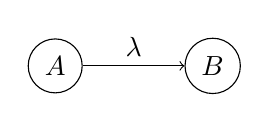
\begin{tikzpicture}
        \node[circle,draw] (s1) at (0, 0) {$A$};
        \node[circle,draw] (s2) at (2, 0) {$B$};
        \draw[->] (s1) to node[above] {$\lambda$} (s2);
    \end{tikzpicture}
\end{figure}

We have two properties:

$$
\sum_{n=0}^{\infty} P_n(t) = 1
$$

$$
\lim_{t \to \infty} P_n(t) = 0 \quad \forall n \geq 0
$$

---

\begin{figure}[H]
    \centering
    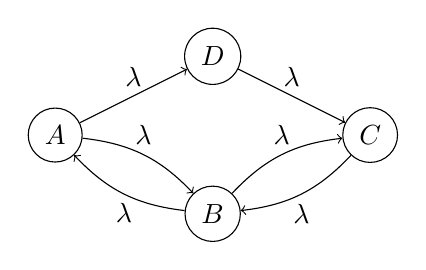
\begin{tikzpicture}
        \node[circle,draw] (s1) at (0, 0) {$A$};
        \node[circle,draw] (s2) at (2, -1) {$B$};
        \node[circle,draw] (s3) at (4, 0) {$C$};
        \node[circle,draw] (s4) at (2, 1) {$D$};
        \draw[->] (s1) to[bend left=20] node[above] {$\lambda$} (s2);
        \draw[->] (s2) to[bend left=20] node[below] {$\lambda$} (s1);
        \draw[->] (s1) to node[above] {$\lambda$} (s4);
        \draw[->] (s2) to[bend left=20] node[above] {$\lambda$} (s3);
        \draw[->] (s3) to[bend left=20] node[below] {$\lambda$} (s2);
        \draw[->] (s4) to node[above] {$\lambda$} (s3);
    \end{tikzpicture}
\end{figure}

To solve a general case, we need to solve the following system of equations:

$$
\dot P = A(t) P
$$

we have:

$$
A_{ij} = \lambda(t) \alpha_{ij}
$$

$$
\dd \theta = \lambda(t) \dd t
$$

$$
\dfrac{\dd \theta}{\dd t} = \lambda(t)
$$

$$
\theta = \int_0^t \lambda(s) \dd s = L(t)
$$

$$
\dfrac{\dd P}{\dd t} = \lambda(t) \alpha P
$$

So:

$$
P(t) = e^{\lambda(t) \alpha} P(0)
$$

---

Let's consider now a case where we have a periodic 

$$
A(t) = \begin{cases}
    A_1 & 0 < \text{mod}(t, T) < Q\\
    A_2 & Q < \text{mod}(t, T) < T
\end{cases}
$$

$$
t = 0 \quad \Rightarrow \quad P(0) = P_0
$$

$$
0 < t < Q
\quad \Rightarrow \quad
\dot P = A_1 P
\quad \Rightarrow \quad
P(t) = e^{A_1 t} P_0
$$

$$
Q < t < T
\quad \Rightarrow \quad
\dot P = A_2 P
\quad \Rightarrow \quad
P(t) = e^{A_2 (t - Q)} P(Q)
$$

$$
T < t < T + Q 
\quad \Rightarrow \quad
\dot P = A_1 P
\quad \Rightarrow \quad
P(t) = \underbrace{e^{A_2 (T - Q)} e^{A_1 Q}}_{B(T,Q)} P(0)
$$

so

$$
\begin{array}{l}
P(T) = B(T,Q) P(0)
\\[0.5em]
P(2T) = B^2(T,Q) P(0)
\\[0.5em]
P(nT) = B^n(T,Q) P(0)
\end{array}
$$

---

CTMC model:

$$
f = \{\sigma_1, \dots, \sigma_n\}
$$

$$
\dot P = A(t) P
$$

$$
P(0) = \left[\begin{array}{c}0\\ \vdots\\1\\ \vdots\\0\end{array}\right] = e_y
$$

---

Gillespie algorithm:

\begin{figure}[H]
    \centering
    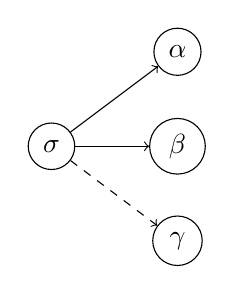
\begin{tikzpicture}[scale=0.8]
        \node[circle,draw] (s1) at (0, 0) {$\sigma$};
        \node[circle,draw] (s2) at (2, 1.5) {$\alpha$};
        \node[circle,draw] (s3) at (2, 0) {$\beta$};
        \node[circle,draw] (s4) at (2, -1.5) {$\gamma$};
        \draw[->] (s1) to (s2);
        \draw[->] (s1) to (s3);
        \draw[->, dashed] (s1) to (s4);
    \end{tikzpicture}
\end{figure}

$$
X(0) = \sigma_0
$$

We want to find when where will be the jump and which will be the next state.

Also in this case we can collapse the states in a single one; the transition rate is given by the sum of the transition rates of the original states.

\begin{figure}[H]
    \centering
    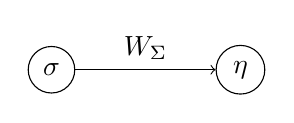
\begin{tikzpicture}[scale=0.8]
        \node[circle,draw] (s1) at (0, 0) {$\sigma$};
        \node[circle,draw] (s2) at (3, 0) {$\eta$};
        \draw[->] (s1) to node[above] {$W_{\Sigma}$} (s2);
    \end{tikzpicture}
\end{figure}

So we can write:

$$
\mathcal P(T) = W_{\Sigma} e ^{- W_{\Sigma} T}
$$

And we have:

$$
t_{n+1} = t_n + T_n, \quad \text{where} \quad T_n \sim \mathcal P(T)
$$


$$
P(\sigma_i) = \Pr(Event (\sigma \to \sigma_i) ara\ t_n + T_n | one E \sim t_n + T_n)
$$

\todo{Che cazzo ha scritto il prof? $\qquad \uparrow\uparrow\uparrow\uparrow\uparrow$}


$$
\Pr\{\sigma \to \sigma_i \ \ (T, T + \dd t)\} \ \ = \ \ (W_x \dd t) e^{-W_{\Sigma}T} \ \ = \ \ \boxed{P(\sigma_i) (W_{\Sigma} e^{W_{\Sigma}T} \dd t)}
$$

\missing{qualcosa}

\dots

\begin{enumerate}
    \item %TODO: write the first point
    
    $$
    T_n \sim W_{\Sigma} e ^{- W_{\Sigma} T}
    \qquad \Rightarrow \qquad
    t_{n+1} = t_n + T_n
    $$ 

    \item %TODO: write the second point
    
    $$
    P(\sigma_i) = \dfrac{W_{\sigma_i}}{W_{\Sigma}} \qquad t_n \to n$$
\end{enumerate}

A first application of the Gillespie algorithm is the following:

\begin{exampleblock}[Gillespie Algorithm: Contagion and Recovery (SIR Model)]
Consider a system with two possible events:
\begin{itemize}
    \item \textbf{Contagion}: $(S, I) \to (S-1, I+1)$, with rate $W_{con} = \beta \dfrac{I}{N} S$
    \item \textbf{Recovery}: $(S, I) \to (S, I-1)$, with rate $W_{rec} = \gamma I$
\end{itemize}

The Gillespie algorithm proceeds as follows:

\begin{enumerate}
    \item \textbf{Initialize}: $t_0 = 0$, $x_0 = (S_0, I_0)$
    \item \textbf{Compute the rates}:
    \begin{itemize}
        \item $W_{con} = \beta \dfrac{I_n}{N} S_n$
        \item $W_{rec} = \gamma I_n$
        \item $W_\Sigma = W_{con} + W_{rec}$
    \end{itemize}
    \item \textbf{Draw two random numbers} $U_1, U_2 \sim \mathcal{U}[0,1]$
    \item \textbf{Determine the time to the next event}:\\
        The waiting time $T_n$ is exponentially distributed:
        $$
        T_n = \frac{-\ln U_1}{W_\Sigma}
        $$
        Update the time: $t_{n+1} = t_n + T_n$
    \item \textbf{Determine which event occurs}:\\
        Compute the probabilities:
        $$
        \Pr(\text{contagion}) = \frac{W_{con}}{W_\Sigma}, \qquad
        \Pr(\text{recovery}) = \frac{W_{rec}}{W_\Sigma}
        $$
        If $U_2 < \Pr(\text{contagion})$, a contagion event occurs; otherwise, a recovery event occurs.
    \item \textbf{Update the state}:
    \begin{itemize}
        \item If contagion: $(S_{n+1}, I_{n+1}) = (S_n - 1, I_n + 1)$
        \item If recovery: $(S_{n+1}, I_{n+1}) = (S_n, I_n - 1)$
    \end{itemize}
    \item \textbf{Repeat} from step 2 until $I_n = 0$ or another stopping criterion is met.
\end{enumerate}

\textbf{Note:} The formula for $T_n$ comes from inverting the CDF of the exponential distribution:
\vspace{0.4em}
$$
CDF(T) = 1 - e^{-W_\Sigma T} \implies T = \frac{-\ln(1-U_1)}{W_\Sigma}
$$
Since $U_1$ is uniformly distributed, so is $1-U_1$, and it is common to write $T = \frac{-\ln U_1}{W_\Sigma}$.
\end{exampleblock}


\begin{figure}[H]
    \centering
    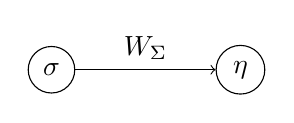
\begin{tikzpicture}[scale=0.8]
        \node[circle,draw] (s1) at (0, 0) {$\sigma$};
        \node[circle,draw] (s2) at (3, 0) {$\eta$};
        \draw[->] (s1) to node[above] {$W_{\Sigma}$} (s2);
    \end{tikzpicture}
\end{figure}

$X(t_n) = \sigma$

$$
\mathcal P(T_n) = W_{\Sigma} (t_n + T) e^{- \int_{t_n}^{t_n + T_n} W_{\Sigma} (z) \dd z}
$$

$$
CDF(T_n) = 1 - e^{- \int_{t_n}^{t_n + T_n} W_{\Sigma} (z) \dd z}
$$

\dots

calling $\Psi(T) = \int_{t_n}^{t_n + T_n} W_{\Sigma} (z) \dd z$

$$
1 - e ^ {-\Psi(T_n)} = U_n \quad \Rightarrow \quad e ^ {-\Psi(T_n)} = 1 - U_n \quad \Rightarrow \quad \Psi(T_n) = - \ln(1 - U_n)
$$

\dots

$$
\beta(t) = \beta_n (1 + \delta \cos(\omega t))
$$

$$
x(t_n) = (S_n, I_n)
$$

$$
\int_{t_n}^{t_n + T_n} W_{\Sigma} (z) \dd z = - \ln(1 - U_n)
$$

$$
\int_{t_n}^{t_n + T_n} \left[
    \gamma I_n + \beta_n \dfrac{I_n}N S_n (1 + \delta \cos(\omega z))
\right] \dd z = - \ln(1 - U_n)
$$

$$
\left[\gamma I_n + \beta_n \dfrac{I_n}N S_n\right]T_n +
\beta_n \dfrac{I_n}N S_n \dfrac{1}{\omega} \left[
\sin(t_n + T_n) - \sin(t_n)
\right]
 = - \ln(1 - U_n)
$$

